
\subsection{NCX Channel Inactivation Model}


\begin{figure}[h!]
 \centering
  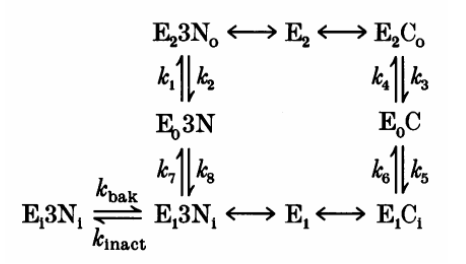
\includegraphics[width=0.5\textwidth]{pic/ncx.png}
 \caption{NCX Ion Channel Model}
 \end{figure}



\subsubsection{Notations}
\begin{itemize}
\item $E_1$ : States with binding sites oriented to the cytoplasmic sides
\item $E_2$ : States with binding sites oriented to the extra-cellular sides
\item $E_{1}3N_{i}$ : States with binding sites oriented to the cytoplasmic sides containing 3 Na+ ions
\item $E_{0}3N$ : States with binding sites occluded with 3 Na+ ions 
\item $E_{2}3N_{0}$ : States with binding sites oriented to the extra cellular sides with 3 Na+ ions
\item $E_{1}C_{1}$ : States with binding sites oriented to the cytoplasmic sides containing 1 Ca++ ion
\item $E_{0}C$ : States with binding sites occluded with 1 Ca++ ion
\item $E_{2}C_{0}$ : States with binding sites oriented to the extra cellular sides with 1 Ca++ ion
\end{itemize}

\newpage

\subsubsection{Simultaneous Diff Equation}



~~~~~~~$\frac{d({E_{2}3N_{o}})}{dt} = k_{1}({E_{0}3N}) - k_{2}({E_{2}3N_{o}})$

$\frac{d({E_{0}3N})}{dt} = k_{7}({E_{1}3N_{i}}) + k_{2}({E_{2}3N_{o}})-(k_{1}+k_{8})(E_{0}3N)$

$\frac{d({E_{1}3N_{i}})}{dt} = k_{bak}({E_{i}3N_{i}}) + k_{8}({E_{o}3N})-(k_{inact}+k_{7})(E_{1}3N_{i})$

$\frac{d({E_{i}3Ni})}{dt} = k_{inact}(E_{1}3N_{i}) - k_{bak}(E_{i}3N_{i}) $

$\frac{d(E_{2}C_{o})}{dt} = k_{4} (E_{o}C) - k_{3}(E_{2}C_{o})$

$\frac{d({EoC})}{dt} = k_{3}(E_{2}Co) + k_{6}(E_{1}C_{i}) - (k_{4} + k_{5}) (E_{o}C)$

$\frac{d({E_{1}C_{i}})}{dt} = k_{5}(E_{o}C) - k_{6}(E_{1}C_{i})$


\subsubsection{Summed Version}

~~~~~~~$\frac{d(E_{1})}{dt} = k_{bak}(E_{i}3N_{i})+ k_{8}(E_{o}3N)+k_{5}(E_{o}C)- (k_{inact}+k_{7}+ k_{6})(E_{1})$

$\frac{d({E_{0}3N})}{dt} = k_{7}(E_{1}) + k_{2}(E_{2})-(k_{1}+k_{8})(E_{o}3N)$

$\frac{d({EoC})}{dt} = k_{3}(E_{2}) + k_{6}(E_{1}) - (k_{4} + k_{5}) (E_{o}C)$

$\frac{d(E_{2})}{dt} = k_{1}(E_{o}3N) + k_{4}(E_{o}C) - (k_{2}+k_{3})E_{2}$

$\frac{d(E_{i}3N_{i})}{dt} = k_{inact}(E_{1})-k_{bak}E_{i}3N_{i}$

$E_{i}3N_{i} = 1 - E_{1} -E_{2} - E_{o}C - E_{o}3N$


\subsubsection{Reduced Equation}

~~~~~~~$\frac{d(E_{1})}{dt} = k_{bak} - k_{bak} E_{2}+(k_{8}-k_{bak})(E_{o}3N)+(k_{5}-k_{bak})(E_{o}C)$

$~~~~~~~~~ - (k_{bak}+k_{inact}+k_{7}+ k_{6})(E_{1})$

$\frac{d({E_{0}3N})}{dt} = k_{7}(E_{1}) + k_{2}(E_{2})-(k_{1}+k_{8})(E_{o}3N)$

$\frac{d({EoC})}{dt} = k_{3}(E_{2}) + k_{6}(E_{1}) - (k_{4} + k_{5}) (E_{o}C)$

$\frac{d(E_{2})}{dt} = k_{1}(E_{o}3N) + k_{4}(E_{o}C) - (k_{2}+k_{3})E_{2}$

\newpage
\subsubsection{Constants}

\begin{itemize}
\item Gamma : $\gamma$ = 0.02
\item Membrane Potential : $Em =... $
\item Kem : $Kem = exp{(0.5\times(1-\gamma)\times Em \times \frac{F}{RT}}) = ....$
\item Rate Constan : $k_{1} = 10^{4} \times Kem$
\item Rate Constan : $k_{2} = F_{3no} \times \frac{10^{4}}{Kem}$
\item Rate Constan : $k_{3} = F_{co} \times 5.17 \times 10^{4} \times Kem$
\item Rate Constan : $k_{4} = 5.17 \times 10^{4}$
\item Rate Constan : $k_{5} = 5.17 \times 10^{4}$
\item Rate Constan : $k_{6} = F_{ci} \times 5.17 \times 10^{4} $
\item Rate Constan : $k_{7} = F_{3ni} \times 1.84 \times 10^{4}$
\item Rate Constan : $k_{8} = 1.84 \times 10^{4} \times$
\item Rate Constan : $k_{bak} = 0.12 $
\item Rate Constan : $k_{in} = 0.8$
\end{itemize}






